\chapter{Bobine et dipole RL}
\section{La bobine}
\subsection{Def et symbole}
\begin{definition}[Bobine]\label{def:bobine}
    Une bobine est constituée par un enroulement d'un fil autour d'un conducteur.\\
    Symbole : \\
    On a r la resistance interne de la bobine, \(r \sim \text{quelques} \Omega \)\\
    Pour une bobine idéale, \(r = 0 \Omega \) \\
    On a aussi \(L\)  : inductance de la bobine, il s'agit d'une grandeur positive qui ne dépend que de la géomérrie de la bobine.
\end{definition}

\subsection{Modelisation d'une bobine}
% Schéma
\begin{center}
    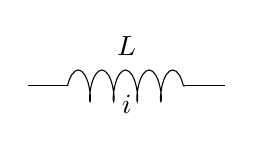
\begin{tikzpicture}
        % Dessin de la bobine
        \draw (0,0) -- (0.5,0);
        \draw[decoration={aspect=0.3, segment length=3mm, amplitude=2mm, coil},decorate] (0.5,0) -- (2,0);
        \draw (2,0) -- (2.5,0);
        % Etiquettes
        \node at (1.25,0.5) {$L$};
        \node[below] at (1.25,0) {$i$};
    \end{tikzpicture}
    \hspace{1cm}
    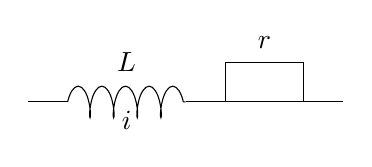
\begin{tikzpicture}
        % Dessin de la bobine avec résistance
        \draw (0,0) -- (0.5,0);
        \draw[decoration={aspect=0.3, segment length=3mm, amplitude=2mm, coil},decorate] (0.5,0) -- (2,0);
        \draw (2,0) -- (2.5,0);
        \draw (2.5,0) rectangle (3.5,0.5);
        \draw (3.5,0) -- (4,0);
        % Etiquettes
        \node at (1.25,0.5) {$L$};
        \node[below] at (1.25,0) {$i$};
        \node at (3,0.75) {$r$};
    \end{tikzpicture}
\end{center}
On peut montrer que : 
\[
    U_{AB} = L \frac{di}{dt} + ri
\]
Le terme \(\frac{di}{dt}\) est caractéristique d'une bobine. 

\subsection{Exploitation de la relation}

On suppose que \(\approx 0 \Omega \implies U_{AB} = L\frac{di}{dt}\).\\
\begin{enumerate}
    \item Si \(i(t) \uparrow \implies \frac{di}{dt} >0 \implies  U_{AB} >0\)
    \item Si \(i(t) \downarrow \implies \frac{di}{dt}<0 \implies U_{AB}<0\)
    \item Plus l'intensité varie rapidement dans le circuit, plus \(\lVert U_{AB} \rVert \) aux bornes de la bobine est élevée.   
\end{enumerate} 

\subsection{Puissance et énergie aux bornes d'une bobine idéale}
Par définition, on a : \(p(t) = U(t) \cdot i(t)\)
\begin{align}
    p(t) &= u(t) \cdot i(t)\\
    &= L \frac{di}{dt} \cdot i(t) \\
    &= \frac{d}{dt}\left[ \frac{1}{2} Li^{2}(t) \right]\\
    &= \frac{dE_{U}}{dt}
\end{align} 

L'énergie emgasinée par la bobine est donc:
\[
    E_{U}(t) = \frac{1}{2}Li^{2}
\]

Rappel : pour un condensateur on a : \(P(t) = u_{c}(t) \cdot i_{c}(t) = u_{c}(t) \cdot C \frac{dU_{c}}{dt} = \frac{d}{dt}\left[ \frac{1}{2}Cu_{c}^{2}(t) \right]\).\\
La tension est continue alors que l'intensité est discontinue.
\section{Le dipôle RL}

%Schema
à \(t=0s\), on ferme l'intérupteur. D'après la loi des mailles : \(\sum_{k} u_{k}E_{k} = 0 \) le long d'une maille orientée.
\begin{align}
    & \implies E-u_{k}-u_{l} =0 \\ 
    & \iff E = u_{r}+u_{l}\\
    & \iff E = R_{i}(t) + L \frac{di}{dt}\\
    & \iff \frac{di}{dt} + \frac{R}{L} i(t) = \frac{E}{L}
\end{align} 
Or \(U_{l} = L \frac{di}{d} \implies \left[ L \right] = v \times s \times A^{-1}\)\\
et \(U_{r} = Ri \implies \left[ R \right] = V \cdot  A^{-1}\)\\
D'ou on a : \(\left[ \frac{L}{R} \right] = s\)
On pose : \(\tau  = \frac{L}{R}\) 
On a donc : \(\frac{di}{dt}+ \frac{i}{\tau} = \frac{E}{L}\)  
\begin{enumerate}
    \item SSH : \(\frac{di}{dt}+ \frac{i}{\tau} = 0 \implies i_{H}(t) = \lambda e^{-\frac{t}{\tau}}\) 
    \item SP : \(\frac{di}{dt} = 0 \implies i_{P}(t) = \frac{E \tau }{L} = \frac{E}{R}\)
    \item SG : \(i(t) = Ae^{-\frac{t}{\tau}}+\frac{E}{R}\)  
\end{enumerate}   
D'après les CI on a : 
\begin{align}
    i(0) = 0 &\implies 0 = \lambda +\frac{E}{R}\\
    & \implies \lambda  = -\frac{E}{R} \\
    & \implies i(t) = \frac{E}{R}(1-e^{-\frac{t}{\tau }}) 
\end{align}

\begin{center}
    \begin{tikzpicture}
        \begin{axis}[
            axis lines = middle,
            xlabel = {$t$},
            ylabel = {$i(t)$},
            domain=0:5,
            samples=100,
            width=10cm,
            height=6cm,
            grid=both,
            grid style={dotted, gray},
            xmin=0, xmax=5,
            ymin=0, ymax=1.2,
            enlargelimits=true
        ]
            \addplot[blue, thick] {1 - exp(-x)};
        \end{axis}
    \end{tikzpicture}
\end{center}

Que vaut alors la tension? 
\begin{eqnarray*}
    U_{l} = L \frac{di}{dt} \implies U_{l} &= L \frac{d}{dt} \left[ \frac{E}{R}(1-e^{-\frac{t}{\tau}}) \right] \\
    &= \frac{EL}{R} \frac{d}{dt} \left[ 1-e^{-\frac{t}{\tau}} \right]\\
    &= \frac{EL}{R} \cdot \frac{1}{\tau} e^{-\frac{t}{\tau}} (\text{ or } \frac{1}{\tau} = \frac{R}{L})\\
    &= \frac{EL}{R} \cdot \frac{R}{L} e^{-\frac{t}{\tau}}\\
    &= Ee^{-\frac{t}{\tau }}
\end{eqnarray*}

\begin{center}
    \begin{tikzpicture}
        \begin{axis}[
            axis lines = middle,
            xlabel = {$t$},
            ylabel = {$i(t)$},
            domain=0:5,
            samples=100,
            width=10cm,
            height=6cm,
            grid=both,
            grid style={dotted, gray},
            xmin=0, xmax=5,
            ymin=0, ymax=1.2,
            enlargelimits=true
        ]
            \addplot[blue, thick] {exp(-x)};
        \end{axis}
    \end{tikzpicture}
\end{center}

\begin{corollary}[Remarque]\label{rem: Rupture du courrant}
    \(U_{l} = L\frac{di}{dt} \approx L \frac{\Delta i}{\Delta t}\) On suppose que \(i\) passe de \(1A\) à \(0A\) en \(1ms\), \(L \approx 1H\). \\
    \( \implies U_{l} \approx 1 \times (\frac{0-1}{10^{-3}}) \approx -1000V \)   
\end{corollary}

\begin{corollary}[Bobines en série]
    On prend deux bobines en série : \(L_{1}\) et \(L_{2}\) avec aux bornes des tensions \(U_{1}\) et \(U_{2}\). On cherche la bobine \(L_{eq}\), avec aux bornes la tension \(U\), équivalente aux deux bobines en série. On a : \(U = U_{1} + U_{2} = L_{1} \frac{di}{dt}+ L_{2} \frac{di}{dt} = (L_{1}+L_{2})\frac{di}{dt}\). D'ou on a : \(L_{eq} = L_{1}+L_{2}\)    
\end{corollary}

\begin{corollary}[Bobines en dérivation]
    On prend deux bobines en dérivation : \(L_{1}\) et \(L_{2}\) traversées par des intensités \(i_{1}\) et \(i_{2}\). On cherche la bobine \(L_{eq}\), traversée par une intensité \(i\), équivalente aux deux bobines en dérivation. On a : \(U = U_{1} = U_{2}\) 
    \begin{eqnarray*}
       &i = i_{1} + i_{2} \\
       &\implies \frac{U}{L_{eq}} = \frac{di}{dt} = \frac{d i_{1}}{dt} + \frac{d i_{2}}{dt} = \frac{U_{1}}{L_{1}} + \frac{U_{2}}{L_{2}} = (\frac{1}{L_{1}} + \frac{1}{L_{2}})U\\
       &\implies \frac{1}{L_{eq}} = \frac{1}{L_{1}} + \frac{1}{L_{2}}
    \end{eqnarray*}     
\end{corollary}
